
%---------------------------------------------------------------------------%
\frame{
\frametitle{Continuous Uniform Distribution}
A random variable X is called a continuous uniform random variable over the interval $(a,b)$ if it's probability density function is given by
\[ f_{X}(x) = { 1 \over b-a} \hspace{1cm} \mbox{ when } a \leq x \leq b \mbox{     (otherwise } f_X(x) = 0 ) \]
The corresponding cumulative density function is
\[ F_x(x) = { x-a \over b-a} \hspace{1cm} \mbox{ when } a \leq x \leq b\]
}
%----------------------------------------------------------------------------------------------------%
\begin{frame}
\frametitle{The Continuous Uniform Distribution}

\vspace{-0.5cm}

\begin{center}
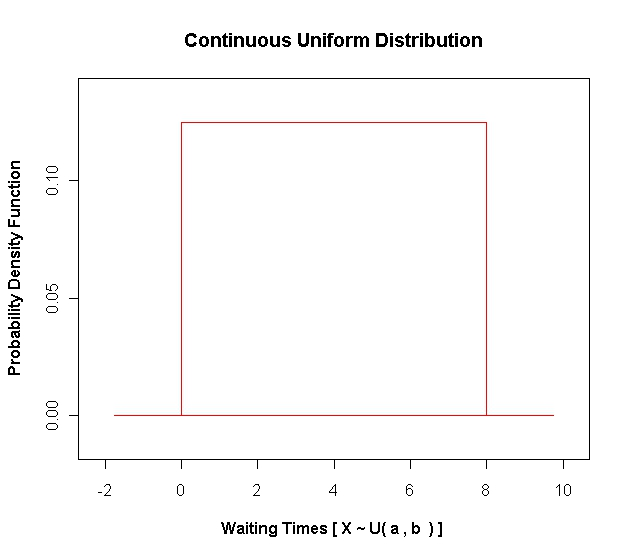
\includegraphics[scale=0.35]{images/6AUniform}

\end{center}
\end{frame}
%---------------------------------------------------------------------------%

%---------------------------------------------------------------------------------------------------------%
\frame{
\frametitle{Uniform Distribution: Cumulative Distribution}
\begin{itemize}

\item For any value ``c" between the minimum value a and the maximum
value $b$, we can say
\item $P(X \geq c)$ \[P(X \geq c) = {b-c \over b-a}\]
here $b$ is the upper bound while $c$ is the lower bound
\item $P(X \leq c)$ \[P(X \leq c) = {c-a \over b-a}\]
here $c$ is the upper bound while $a$ is the lower bound.
\end{itemize}
}

%-----------------------------------------------------------------------------%
\frame{
\frametitle{Uniform Distribution: Mean and Variance}
\begin{itemize}
\item The mean of the continuous uniform distribution, with parameters $a$ and $b$ is
\[ E(X) = {a+b \over 2}\]
\item The variance is computed as
\[ V(X) = {(b-a)^2 \over 12}\]
\end{itemize}
}
